\documentclass{beamer}[10pt, usepdftitle=false, handout]

\beamertemplatenavigationsymbolsempty

\usepackage[T1]{fontenc}
\usepackage[]{algorithm2e}
\usepackage{multimedia}
\usepackage{gensymb}
\usepackage{textcomp}

%\usepackage[font=small,labelfont=bf]{caption} 

\usetheme{Boadilla}

\title{Basic of Computer Networks 1}
\author[]{Paul Blondel}
\institute[]{CNAM}
\date[]{March 1st, 2019}

\usepackage[style=british]{csquotes}


\def\signed #1{{\leavevmode\unskip\nobreak\hfil\penalty50\hskip1em
  \hbox{}\nobreak\hfill #1%
  \parfillskip=0pt \finalhyphendemerits=0 \endgraf}}

\newsavebox\mybox
\newenvironment{aquote}[1]
  {\savebox\mybox{#1}\begin{quote}\openautoquote\hspace*{-.7ex}}
  {\unskip\closeautoquote\vspace*{1mm}\signed{\usebox\mybox}\end{quote}}


\setbeamertemplate{headline}
{
  \leavevmode%
  \hbox{%
  \begin{beamercolorbox}[wd=1.0\paperwidth,ht=2.25ex,dp=1ex,center]{author in head/foot}%
    \usebeamerfont{author in head/foot}\insertsubsection
  \end{beamercolorbox}}%
  \vskip0pt%
}


\setbeamertemplate{footline}
{
  \leavevmode%
  \hbox{%
  \begin{beamercolorbox}[wd=.5\paperwidth,ht=2.25ex,dp=1ex,center]{author in head/foot}%
    \usebeamerfont{author in head/foot}\insertsection
  \end{beamercolorbox}%
  \begin{beamercolorbox}[wd=.5\paperwidth,ht=2.25ex,dp=1ex,center]{title in head/foot}%
    \usebeamerfont{title in head/foot} \inserttitle \hspace*{2em}  \insertframenumber{} / \inserttotalframenumber\hspace*{2ex} 
  \end{beamercolorbox}}%
  \vskip0pt%
}

\AtBeginSection[]
{
   \begin{frame}
    \tableofcontents[ 
    currentsection] 
   \end{frame}
}

\begin{document}
	{
	\setbeamertemplate{footline}{
  	\leavevmode%
  	\hbox{%
  	\begin{beamercolorbox}[wd=.5\paperwidth,ht=2.25ex,dp=1ex,center]{author in head/foot}%
  	\end{beamercolorbox}%
  	\begin{beamercolorbox}[wd=.5\paperwidth,ht=2.25ex,dp=1ex,center]{title in head/foot}%
  	\end{beamercolorbox}}%
  	\vskip0pt%	
	} 
	\begin{frame}
	\titlepage
	\end{frame}

	\begin{frame}
	
	\begin{aquote}{Tim-Bernes Lee - Creator of the WEB}
I think, in general, it's clear that most bad things come from misunderstanding, and communication is generally the way to resolve misunderstandings — and the Web's a form of communications — so it generally should be good.
	\end{aquote}	
	
	\end{frame}


	\begin{frame}
		\tableofcontents
	\end{frame}
	}

	\addtocounter{framenumber}{-3}

	\section{Introduction}	

    \begin{frame}[label=(first)]
	
	\begin{block}{Nowadays}
	The latest progresses in Signal Progressing and the recent convergence of techniques permitted the rapid democratization of data transfer around the world. This is the Web and the Internet!
	\end{block}
	\vspace*{1em}
	
	But first let's talk about a simple communication case between two machines: 
	\vspace*{1em}
	
	\begin{center}
	\begin{figure}
		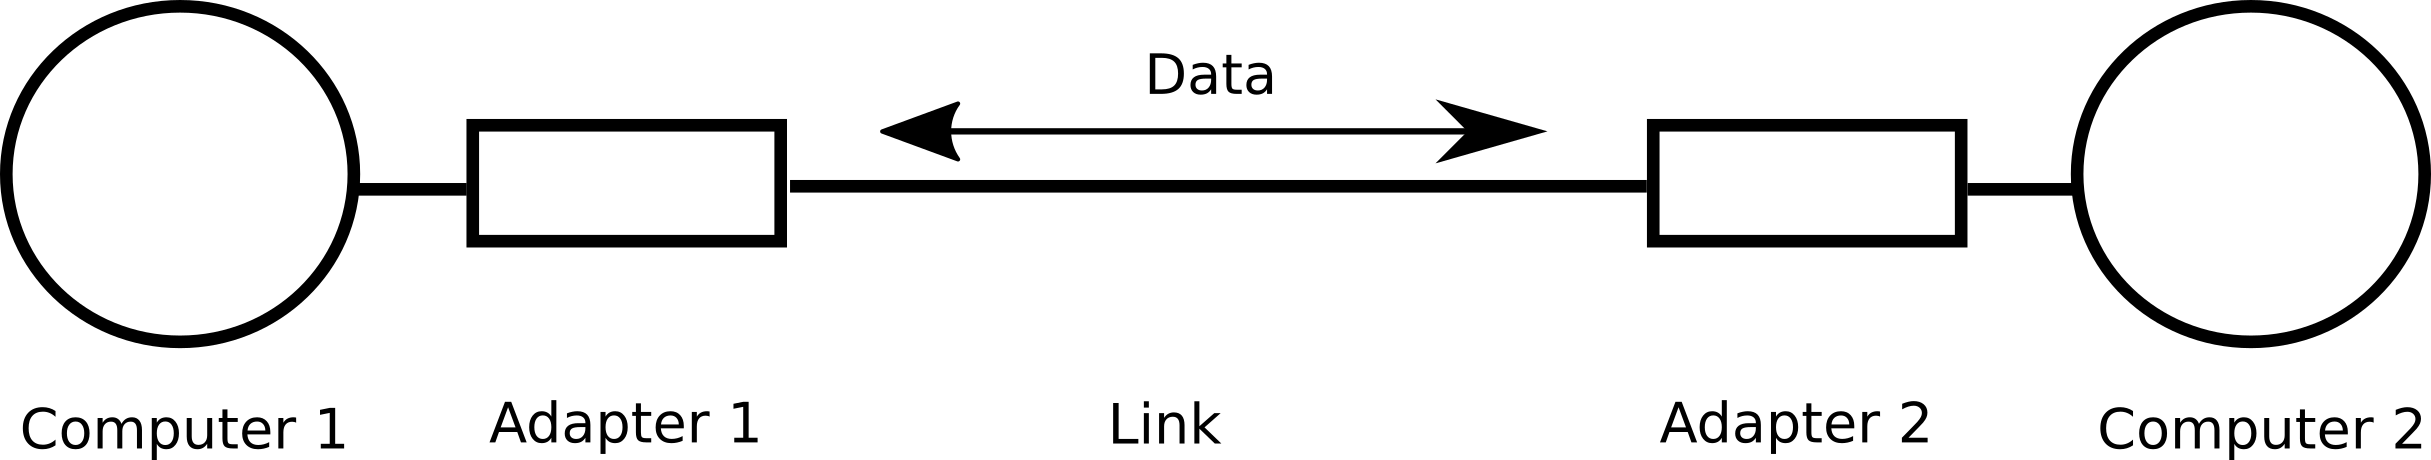
\includegraphics[scale=0.2]{images/link_computer.png} 
     	%\vspace*{-0.5em}
		%\caption{Floating gate transistor cell}
	\end{figure}	
	\end{center}
	 

			
    \end{frame}

	\begin{frame}
	
	\begin{block}{Principle}
	We need to ensure a reliable transfer of data between a machine 1 and a machine 2.
	\end{block}	
	\vspace*{1em}
	
	This requires several things:
	\vspace*{1em}
	
	\begin{enumerate}
	\item{Data must be translated into something both machines can understand and process (= a same language)}
	\item{There must be a link between the machines (= a cable, radio signals, etc.)}
	\item{The transfer of data should be managed by a protocol to ensure a good communication (= a discussion)}
	\item{A mode of exchange should be defined (= I'm master, I'm slave, we are even, etc.)}	
	\item{An adaptation system must be present between the link and the machine (= a ear)}	
	\end{enumerate}		
		

	\end{frame}

	\section{Notions}
	
	\begin{frame}
		
	Let's first give some notions:
	\vspace*{1em}
	
	\textbf{Bit rate:}
	\vspace*{1em}
	
	In transmission systems a binary representation of the data is employed.
	\vspace*{0.5em}
	
	The bit rate (R) is the number of bits (0s and/or 1s) $V$ transmitted during a specific unit of time $dt$.
	\vspace*{0.5em}
	
	$R = \frac{V}{dt}$
	\vspace*{0.5em}
	
	The higher the bit rate, the more data (bits) are transmitted during an amount of time.

	
	\end{frame}

	\begin{frame}
	
	\textbf{Signal to noise ratio:}
	\vspace*{1em}

	Transmitted signals can be distributed due to electromagnetic phenomena (we call that noise). This disturbance generates errors.
	\vspace*{0.5em}
	
	The ratio between the power of the transmitted signal and the noise is called the signal to noise ratio:
	\vspace*{0.5em}	
	
	$S_{NR} = S_{N_{db}} = 10 \times log_{10}(\frac{S}{N})$
	
	
	
	\end{frame}
	
	\begin{frame}
	
	\textbf{Error rate:} 
	\vspace*{1em}
	
	As mentioned before noise disturbs the transmission and can modify one or several transmitted bits, changing the nature of the transmitted message (this is the \textbf{binary error rate}, or \textbf{error rate}).
	\vspace*{0.5em}
		
	The binary error rate (BER) is: 
	\vspace*{0.5em}
	
	$BER = \frac{number\ of\ erroneous\ bits}{number\ of\ transmitted\ bits}$
		
	
	\end{frame}	
	
	\begin{frame}
	
	\textbf{Time to transfer (or latency):}
	\vspace*{1em}
	
	This measures the time between the emission of q bit at the entry of the network and the reception of a bit at the exit of the network.
	\vspace*{0.5em}
	
	\begin{alertblock}{Not constant!}
	The time of transfer is not constant, it varies with time (depending on the network changes).
	\end{alertblock}
		
	
		
		
	
	\end{frame}	
	
	\begin{frame}
	
	\textbf{Spectral signal:}
	\vspace*{1em}	
	
	Every periodic signal can be decomposed into a sum of elementary sigmoids.
	\vspace*{1em}	
	
	\begin{center}	
	\begin{figure}
		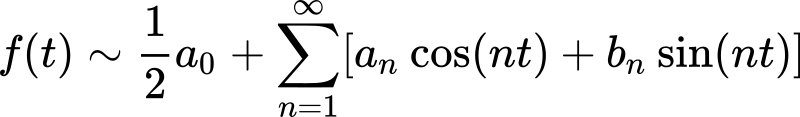
\includegraphics[scale=0.01]{images/fourrier-series.png} 
     	%\vspace*{-0.5em}
		%\caption{Floating gate transistor cell}
	\end{figure}	
	\end{center}
	
	\end{frame}

	\begin{frame}
	
	Types of information:
	\vspace*{1em}
	
	\begin{itemize}
	
	\item{\textbf{Discrete:} assembly of elements independents each other (series of discontinuous values)
		\begin{itemize}
			\item{Example: text is a set of words (composed of letters)}		
		\end{itemize}			
	}
	\item{\textbf{Contiguous:} result of the contiguous variation of a physical phenomenon 
		\begin{itemize}
			\item{Example: analogical signal (can take an infinite range of values)}		
		\end{itemize}			
	 }	
	
	\end{itemize}		
	
	\end{frame}	
	
	\begin{frame}
	
	To be processed, information need to be \textit{translated into bits}. Every part of information is translated into a string of bits. This operation is called \textbf{encoding the information}. 
	\vspace*{0.5em}
	
	
	Encoding the information consists in matching symbols to binary representations (code words).
	\vspace*{0.5em}
	
	In the given example below the information is made of alphanumerical characters\footnote{it is a bijection}:	
		\vspace*{1em}
	
	\begin{center}	
	\begin{figure}
		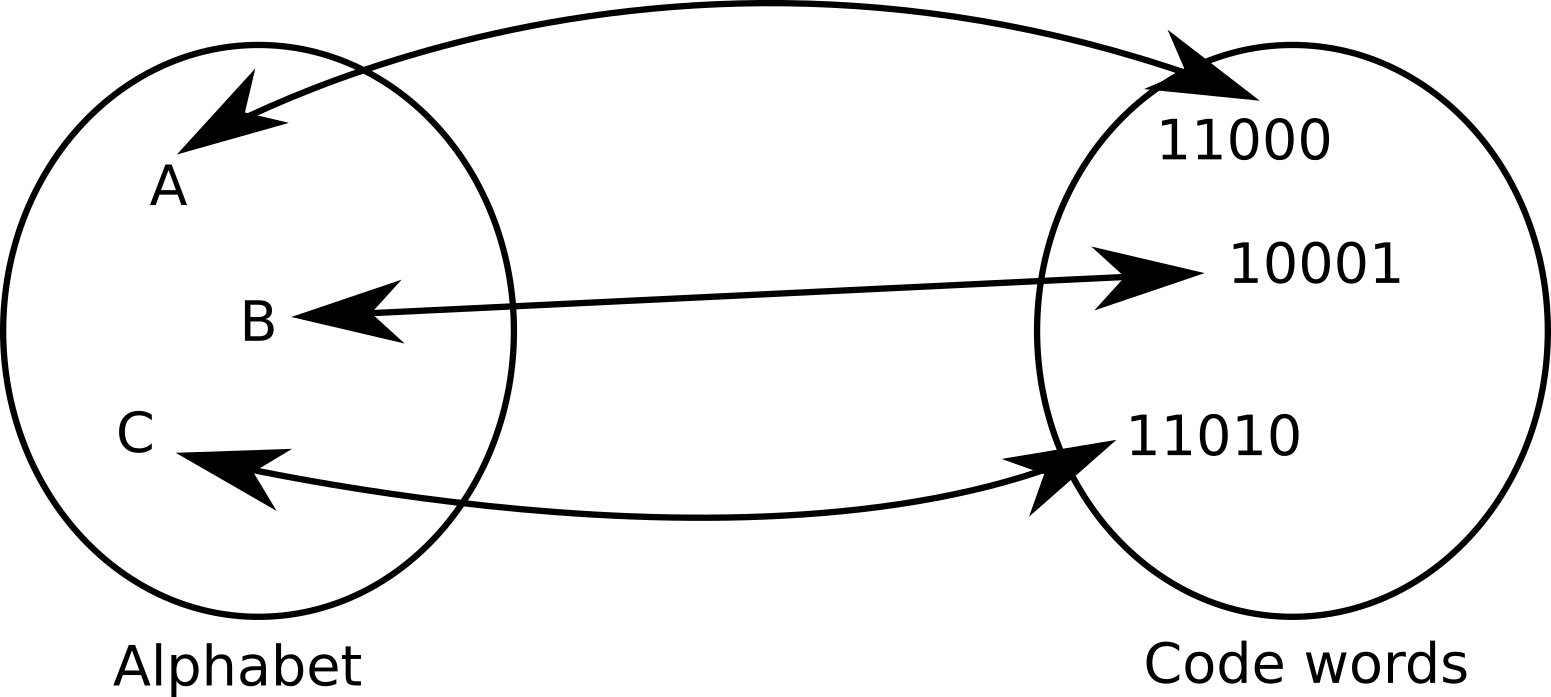
\includegraphics[scale=0.3]{images/encoding.png} 
     	%\vspace*{-0.5em}
		%\caption{Floating gate transistor cell}
	\end{figure}	
	\end{center}
		
	\end{frame}

	\section{Encoding the information}
	\subsection{Different types of coding}

	\begin{frame}
	
	\textbf{Different types of code:}	
	\vspace*{1em}	
	
	Coding the different states of a system can be done by two approaches. Giving two types of code:
		\vspace*{1em}	
	
	\begin{itemize}
	\item{fix length codes (each state of the system is equivalent)}
	\item{variable length codes (the frequency of occurrence of a state is taken into account)}
	\end{itemize}		
	
	\end{frame}

	\subsection{Fixed-length codes}

	\begin{frame}
	
	Fix-length codes:
			\vspace*{1em}	
	
	\begin{itemize}
	\item{Each state of the system is coded by a certain number of bits (called length of code) with:
		\begin{itemize}
			\item{1 bit: we can code 2 states (0 or 1}
			\item{2 bits: we can code 4 states (00, 01, 10, 11)}
			\item{N bits: we can code $2^N$ states}
		\end{itemize}
	}	
	
	\end{itemize}
	
	The number of states required to code $P$ states is $n$ such as: 
	$2^{(n-1)} < P \leq 2^n$  	
		\vspace*{1em}	
	
	Example: We have 26 letters in the alphabets, how many bits are necessary to code $P$ values?
	We need 5 bits, because: $2^4 < 26 \leq 2^5$	
	
	
	\end{frame}
	
	\begin{frame}
	
	Another notion is the quantity of information $Q$:
		\vspace*{1em}	

	$Q = log_2(\frac{1}{p})$
		\vspace*{1em}	
	
	For example, if we consider we have an equal probability of having all the letters of the alphabet (26 letters), the probability of having one letter is $\frac{1}{26}$, so we have the following quantity of information (expressed in bits, or shannon):
		\vspace*{1em}	

	
	$Q = log_2(26) = 4.66$ bits (or shanon)
		\vspace*{1em}	
	
	\begin{block}{Quantity of information}
	The quantity of information is the optimal length in bits of a code word (if we have an equal probability) 
	\end{block}
		
	\end{frame}	

	\begin{frame}

	Examples of character encoding systems:
		\vspace*{1em}	
	
	\begin{itemize}
	
	\item{The \textbf{Baudot code} is encoded on 5 bits. With the Baudot code we can code up to 32 characters (and thus the 26 letters of the alphabet).}
	\item{The \textbf{ASCII table} (7 bits encoding). With the ASCII table uppercase letters, system and special characters can also be encoded (we can code 128 characters).}
	
	\end{itemize}
	
		
	\begin{center}	
	\begin{figure}
		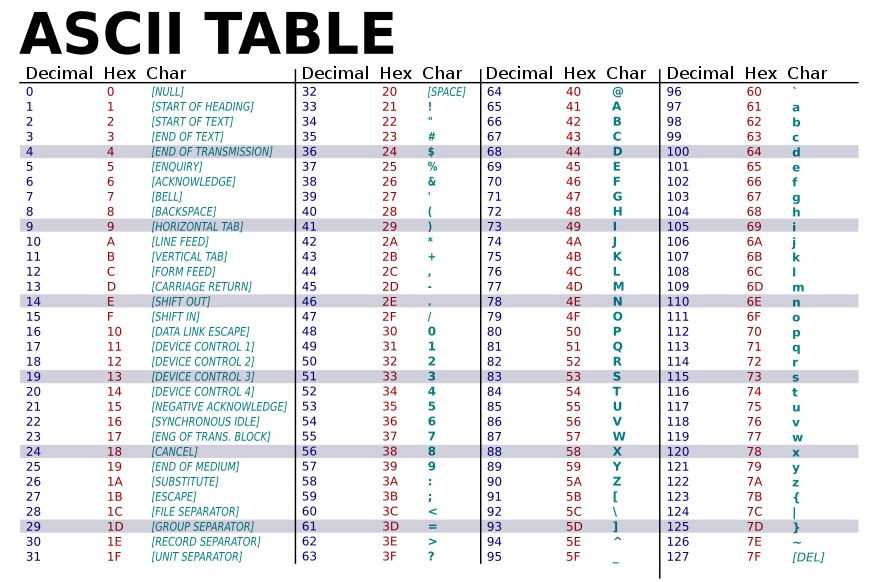
\includegraphics[scale=0.2]{images/ascii_table.png} 
     	%\vspace*{-0.5em}
		%\caption{Floating gate transistor cell}
	\end{figure}	
	\end{center}
	 
		
	
	
	\end{frame}

	\subsection{Variable-length codes}

	\begin{frame}
	
	In case the states of the system have not an equal probability to occur, we compute an average quantity of information (this is called the entropy).
		\vspace*{1em}	
	
	The average quantity of information is called entropy and is given by this formula:
		\vspace*{1em}	
	
	$H=\sum{}_{i=1}^{i=n}(p_i\times log_2(\frac{1}{p_i}))$
		\vspace*{1em}	
	
	The entropy is the optimal length for coding the symbols of the system.
		\vspace*{1em}	
	
	\end{frame}
	
	\begin{frame}	
	
	Example:
		\vspace*{1em}	
	
	\begin{tabular}{|c|c|} 
	\hline
	\textbf{state} & \textbf{probability of occurrence} \\ \hline
	C & 0.48 \\ \hline
	N & 0.21 \\ \hline
	A & 0.12 \\ \hline
	M & 0.08 \\ \hline
	D & 0.06 \\ \hline
	G & 0.05 \\ \hline
	\end{tabular}	
		\vspace*{1em}	
		
	$H=-(0.48\times log_2(0.48) + 0.21\times log_2(0.21) + 0.12\times log_2(0.12) + 0.08\times log_2(0.08) + 0.06\times log_2(0.06) + 0.05\times log_2(0.05))=1.92$ bits
		\vspace*{1em}	
	
	The optimal code is 1.92 bits (with a fixed length code it would have been 3 bits)	
	
	
	\end{frame}

	\subsection{ASCII to unicodes}

	\begin{frame}
	
	\textbf{ASCII to unicodes:}
		\vspace*{1em}	
	
	With ASCII we can code only 128 characters...
		\vspace*{0.5em}	
	
	With ISO-8859-X (coded on 8bits) other 128 characters can be used to code for other characters (because of the 8-th bit). Other characters specific to languages such as: latin, cyrillic, arabic, greek and hebrew can be encoded as well. 
	\vspace*{0.5em}		
		
	Example of ISO-8859-X unicode: ISO-8859-1.
	\vspace*{0.5em}	
	
	With ISO-8859-X unicodes it's not possible to encode Chinese characters. The Guobiao character encoding permits that (for simplified characters: GB2312, GB13000, GB18030, GBK, GB\_1988-80 and GB\_198880, for traditional characters:  BIG-5, BIG-FIVE, BIG5-HKSCS, BIG5, BIG5HKSCS, BIGFIVE, CN-BIG5, CN-GB and CN).		
		
	
	\end{frame}

	\subsection{Dealing with contiguous information}

	\begin{frame}
	
	Contiguous information:
	\vspace*{1em}	
	
	A contiguous signal (can be made from an analogous sensor for instance) has to be transformed into a string of bits to be transferred. The signal needs to be digitized.   
	\vspace*{0.5em}	
	
	The digitization of a contiguous signal can be made by extracting samples at regular times:
	\vspace*{0.5em}	
	
	\begin{itemize}
	\item{The sampling interval is constant (= having a fixed sampling frequency)}
	\item{The order of magnitude is kept}
	\item{Each sample is encoded in binary}
	\end{itemize}
	
	\end{frame}
	
	\begin{frame}	
	
	\begin{center}	
	\begin{figure}
		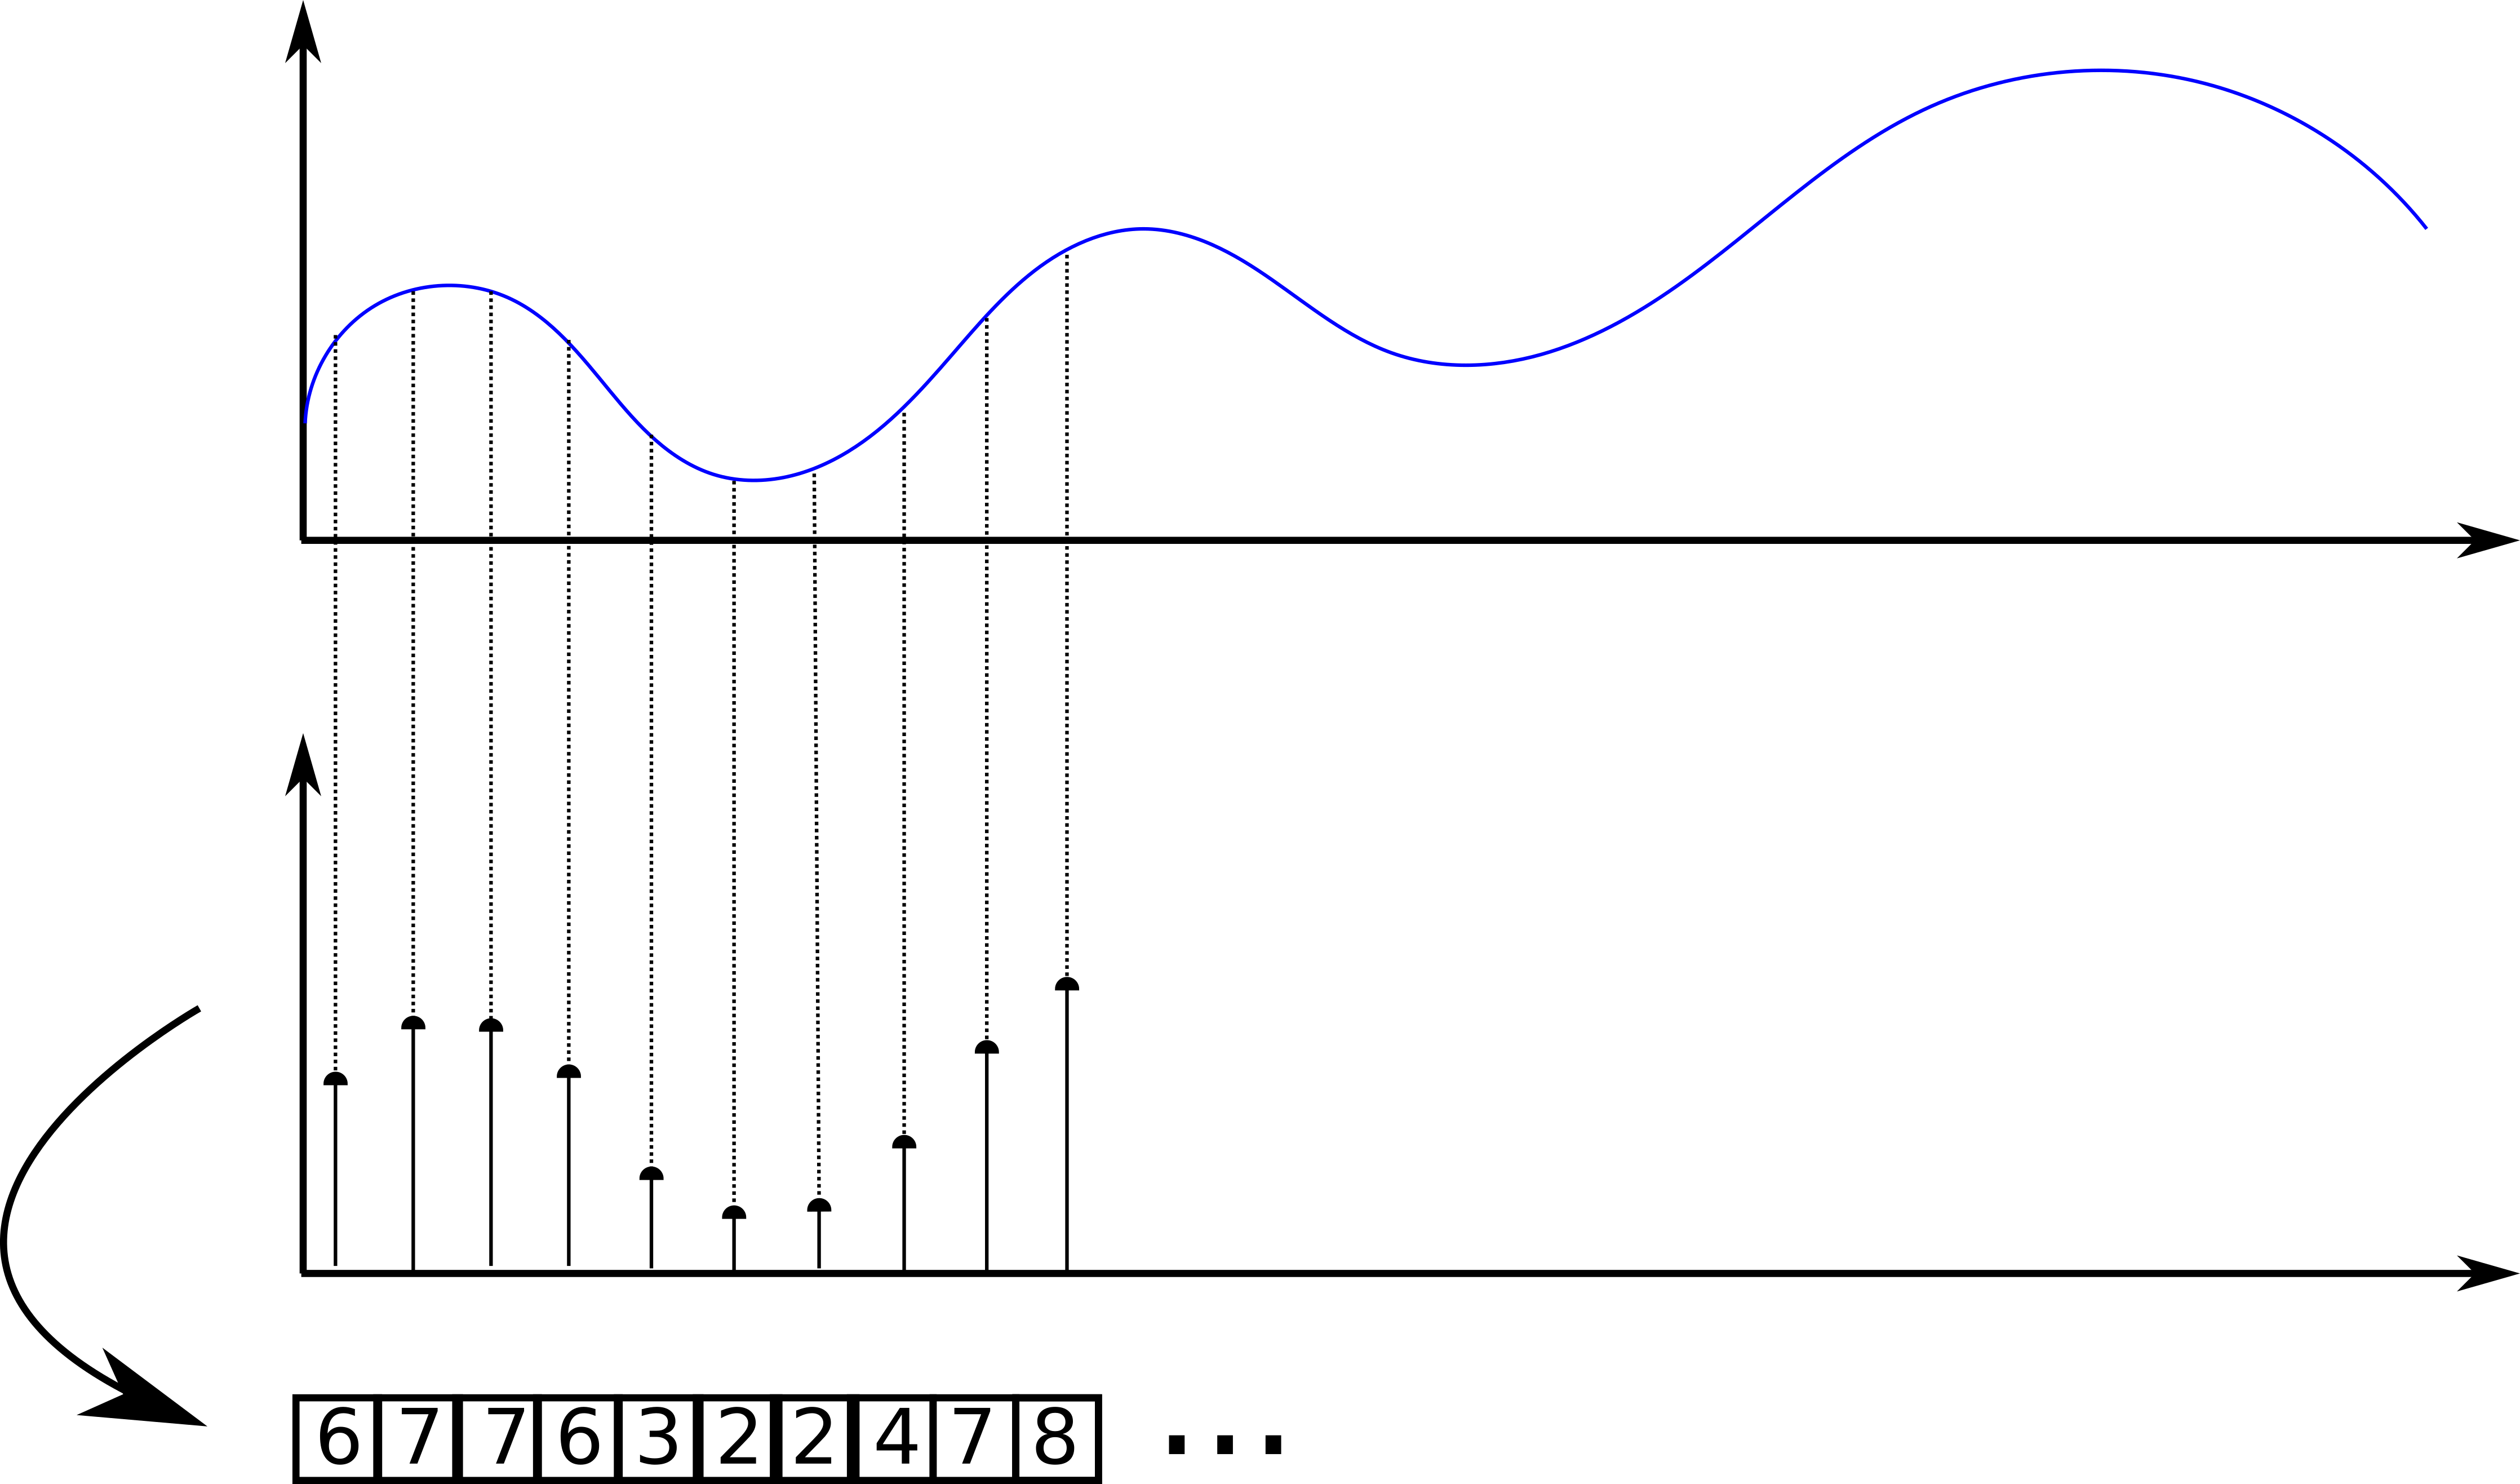
\includegraphics[scale=0.1]{images/digit.png} 
     	%\vspace*{-0.5em}
		%\caption{Floating gate transistor cell}
	\end{figure}	
	\end{center}
	\vspace*{0.5em}	
	 
	
	
	\begin{alertblock}{Beware}
	Shannon Law: the \textbf{sampling frequency must be bigger or equal to twice the maximum frequency of the signal}.	
	\end{alertblock}
		
	
	\end{frame}

	\begin{frame}
	
	Example 1:
	\vspace*{1em}	
	
	The max frequency of the human voice is between 300Hz and 3400Hz.
	\vspace*{0.5em}	
	
	Let's choose $F_{max}=$4000Hz
	\vspace*{0.5em}	
	
	According to the Shannon law, $F_{sampling}$ must be $\geq 2\times F_{max}$
	\vspace*{0.5em}	
	
	So let's choose $F_{sampling}=$8000Hz (8000 samples per seconds)
	\vspace*{0.5em}	
	
	Besides, to get a correct audio reproduction each sample should be encoded on 12 bits.
	\vspace*{0.5em}	
	
	So the Bit Rate should be: $8000\times 12=$ 96000 bits/second 	
	\vspace*{0.5em}	
	
		
	\end{frame}

	\begin{frame}

	Example 2:
	\vspace*{1em}	
	
	As you know, the color can be decomposed into three different primary colors (red, green and blue).
	\vspace*{0.5em}	
	
	The weighted sum of these three primary colors give the color (this is the additive synthesis).
	\vspace*{0.5em}	
	
	 \begin{center}	
	\begin{figure}
		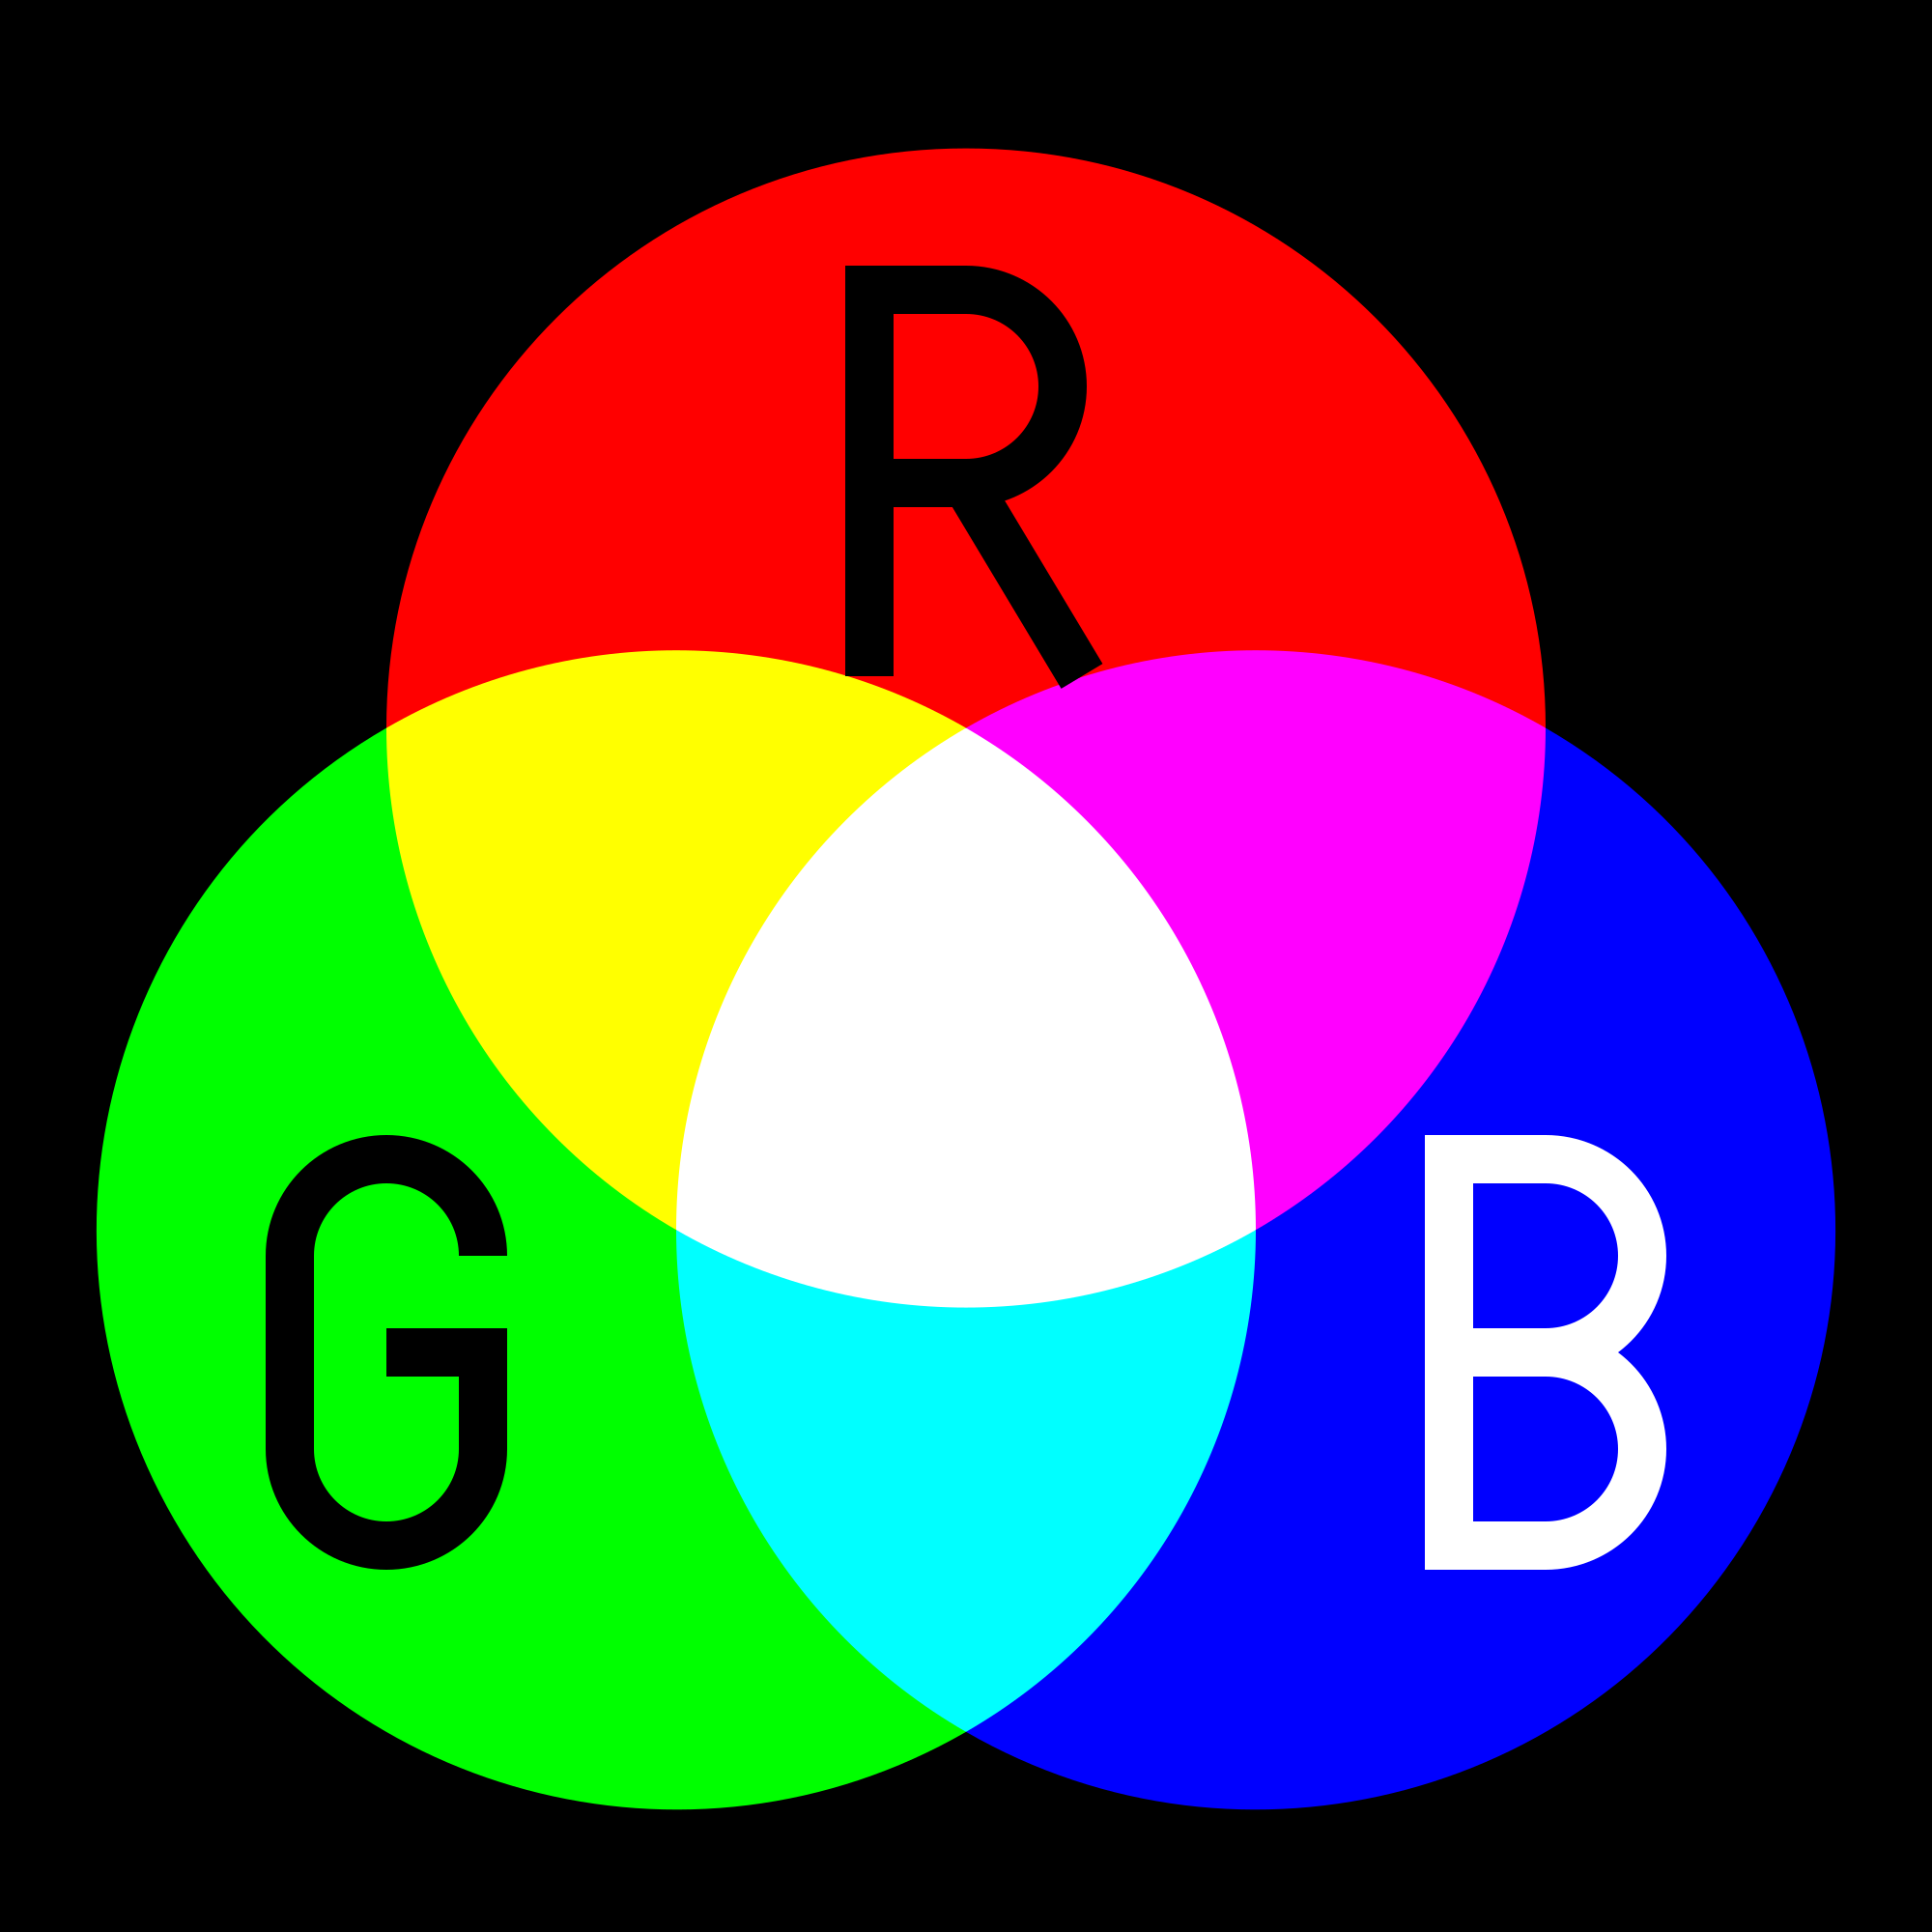
\includegraphics[scale=0.05]{images/additive.png} 
     	%\vspace*{-0.5em}
		%\caption{Floating gate transistor cell}
	\end{figure}	
	\end{center}
	
	
	\end{frame}

	\begin{frame}
	
	Each image point in an image is represented  by two values: the luminance (luminious intensity) and the chrominance (conveying color information).
	\vspace*{1em}	
	
	
	These two values are bounded together by this relation:
	\vspace*{0.5em}		
	
	$Y=0.3\times R + 0.59\times V + 0.11\times B$
	\vspace*{0.5em}	
	
	Y: luminance
	R, G and B: chrominance components
	\vspace*{0.5em}	
		
		
	For example, with the lowest quality of European Digital TV standard we have:
	\vspace*{0.5em}	
	
	\begin{itemize}
	\item{625 lines per image (576 lines are really used).}
	\item{720 points per line}
	\item{25 images/second}	
	\end{itemize}			
	\vspace*{0.5em}	
		
	In this format only the luminance (for retro-compatibility with old monochrome TVs) and the red and blue chrominance components are transmitted (actually knowing these three values permit to guess the green component pretty easily). 	
	
	\end{frame}
	
	\begin{frame}
	
		
	Thus we transmit:	
	\vspace*{1em}	
		
	\begin{itemize}
	\item{720 points per line for the luminance (encoded on 8bits)}
	\item{360 points each for the blue and red chrominance (encoded on 8bits)}
	\end{itemize}	
	\vspace*{0.5em}		
	
	So we have 1440 points per line.
	\vspace*{0.5em}	
	
	Number of bits to transmit for one image = $(1440\times 8\times 576)	= 6635520$ bits
	\vspace*{0.5em}	
	
	With a framerate of 25 images/second:
	The Bit Rate must be: $6635530\times 25=166$Mbit/s
	\vspace*{0.5em}	
		
	Actually this Bit Rate is difficult to realize \, one solution is to compress the data to lower the required Bit Rate.
	
	This is the goal of the "Motion Picture Expert Group" or MPEG: they define the compression algorithm for sound and video.		
		
	\end{frame}

	\section{Compressing the data}

	\subsection{Useful for what?}
	\begin{frame}
	
	In many cases a too high Bit Rate is not always doable: the cost to produce a high Bit Rate may be too expensive regarding the application or it may be technological difficult to realize. 
	\vspace*{0.5em}	
	
	In order to reduce the required Bit Rate while keeping the same semantic: the data can be compressed.\vspace*{0.5em}	
	
	There are two kinds of compression algorithms: 
	\vspace*{1em}	

	\begin{itemize}
	\item{Reversible algorithms: data can be restored identically after decompression}
	\item{Irreversible algorithms: data is not identically restored after decompression (but the semantic is kept)}
	\end{itemize}

	\end{frame}

	\subsection{Some notions}

	\begin{frame}
	
	The compression efficiency can be gauged using three formulas:
	\vspace*{1em}	
	
	\begin{itemize}
	\item{The compression coefficient C}
	\item{The compression rate R (invert of the compression coefficient)}
	\item{The compression gain G (in percents)}	
	\end{itemize}	
	\vspace*{1em}		
	
	$C=\frac{size\ before\ compression}{size\ after\ compression}$
	
	$R=\frac{1}{C}$
	
	$G=(1-R)\times 100$	
		
	\end{frame}	


\end{document}